%!TEX root = ../dispense_QP.tex

\chapter{Il caso dell'oscillatore armonico}
Siamo ora pronti ad analizzare uno dei pilastri su cui si fonda non solo la fisica classica, bensì anche la meccanica quantistica: il caso dell'\textbf{oscillatore armonico}. Le potenzialità che contraddistinguono questo concetto sono pressochè infinite, dall'analisi di semplici moti armonici alla discussione sulla quantizzazione del campo magnetico. 

L'hamiltoniana del sistema in una dimensione\footnote{La restrizione unidimensionale non toglie generalità al sistema, eventualmente estendibile al caso tridimensionale.}, classicamente, risulta:
\[
    \mathcal{H} = \frac{{p}^2}{2m} + \frac{1}{2}m\omega^2x^2 \quad, 
\] 
con $\omega$ la pulsazione del sistema e $m\omega^2$ la sua \emph{costante elastica}. Effettivamente, un sistema con un potenziale dalla forma funzionale generica può essere ben approssimato, nell'intorno di un suo minimo (ovvero un punto di equilibrio stabile), da un polinomio di secondo grado:
\[
\begin{aligned}
    U(x) &= U(x_0) + \underbrace{U'(x_0)(x-x_0)}_{\text{0 nel punto di equilibrio}} + \frac{1}{2}U''(x_0)(x-x_0)^2 + o(x-x_0)^2 \\
    &\approx U(x_0) + \frac{1}{2}U''(x_0)(x-x_0)^2 \quad.
\end{aligned}
\]
È dunque fondamentale proporre una riformulazione quantistica che, per di più, è sufficientemente banale. Assumendo conto di un hamiltoniana formata dall'operatore energia cinetica e dall'operatore energia potenziale elastica. La S.E. stazionaria risulta:
\[
    \h{H}\psi(x) = \left( -\frac{\hbar^2}{2m}\dv[2]{}{x} + \frac{1}{2}m\omega^2x^2 \right)\psi(x) = E\psi(x) \quad.
\]
La soluzione di questa equazione differenziale è particolarmente complicata è coinvolge la \emph{teoria dei polinomi ortogonali di Hermite}. Noi sfrutteremo un metodo non puramente algebrico, detto \textbf{metodo dell'algebra generatrice dello spettro}, che ci semplificherà notevolmente la vita... il risultato che otterremo sarà comunque identico a quello previsto dalla teoria dei polinomi di Hermite, della quale daremo una breve introduzione al termine di questo capitolo.

\section{Il metodo dell'algebra generatrice dello spettro}
L'idea che implementeremo è quella di sfruttare le proprietà algebriche dell'hamiltoniana dell'oscillatore armonico per definire due nuovi operatori: l'\textbf{operatore di creazione} $\hat{a}$ e l'\textbf{operatore di annichilazione} $\hat{a}^\dagger$. Nell'algebra di base, la somma di due quadrati è fattorizzabile come segue:
\begin{equation}
    x^2 + y^2 = x^2 - (iy)^2 = (x+iy)(x-iy) \quad,
    \label{eq:somma_quadrati}
\end{equation}
classica e intramontabile regola della \emph{differenza di quadrati = somma per differenza}. Cerchiamo ora di fare lo stesso con la nostra hamiltoniana: gli operatori coinvolti, posizione e momento, si trovano infatti al grado 2 ma, in generale, dipendenze lineari sono più semplici da analizzare. Prima di partire, notiamo che il prodotto fra operatori, in generale, non è commutativo... dobbiamo riformulare la \eqref{eq:somma_quadrati}:
\begin{equation}
\begin{aligned}
    (\h{A} - i\h{B})(\h{A} + i\h{B}) = \h{A}^2 + \h{B}^2 - i\h{B}\h{A} + i\h{A}\h{B} = \h{A}^2 + \h{B}^2 +i[\h{A},\h{B}] \\
    \implies \h{A}^2 + \h{B}^2 = (\h{A} - i\h{B})(\h{A} + i\h{B}) - i[\h{A},\h{B}] \quad.
\end{aligned}
\label{eq:somma_diff_operatori}
\end{equation}
Vediamo adesso cosa succede provando fattorizzare $\h{H}$, assumendo $\hat{p} = \hat{p}_x$:
\[
\begin{aligned}
    \h{H} = \frac{\hat{p}^2}{2m} + \frac{1}{2}m\omega^2\hat{x}^2 &=  \frac{m\omega^2}{2}\left( \hat{x}^2 + \frac{\hat{p}^2}{m^2\omega^2}  \right) \\
    &\overset{(1)}{=}  \frac{m\omega^2}{2}\left[\left( \hat{x} - i\frac{\hat{p}}{m\omega}  \right)\left( \hat{x} + i\frac{\hat{p}}{m\omega}  \right)-i \frac{[\hat{x}, \hat{p}]}{m\omega}\right] \\
    &= \frac{m\omega^2}{2}\left[\left( \hat{x} - i\frac{\hat{p}}{m\omega}  \right)\left( \hat{x} + i\frac{\hat{p}}{m\omega}  \right)+ \frac{\hbar}{m\omega}\right] \\
    &= \omega\hbar\bigg[\frac{m\omega}{2\hbar}\left( \hat{x} - i\frac{\hat{p}}{m\omega}\right)   \left( \hat{x} + i\frac{\hat{p}}{m\omega}  \right)+ \frac{1}{2}\bigg] \\
    &= \omega\hbar\bigg[\underbrace{\sqrt{\frac{m\omega}{2\hbar}}\left( \hat{x} - i\frac{\hat{p}}{m\omega}  \right)}_{\hat{a}^\dagger} \underbrace{\sqrt{\frac{m\omega}{2\hbar}}\left(\hat{x} + i\frac{\hat{p}}{m\omega}  \right)}_{\hat{a}}+ \frac{1}{2}\bigg] \quad.
\end{aligned}
\]
dove in $(1)$ abbiamo sfruttato la \eqref{eq:somma_diff_operatori}. Definiamo così gli operatori di creazione e annichilazione:
\[
\begin{dcases}
    \hat{a} = \sqrt{\frac{m\omega}{2\hbar}}\left(\hat{x} + i\frac{\hat{p}}{m\omega}\right) \\
    \hat{a}^\dagger = \sqrt{\frac{m\omega}{2\hbar}}\left(\hat{x} - i\frac{\hat{p}}{m\omega} \right)
\end{dcases}
\implies 
\begin{dcases}
    \hat{x} = \sqrt{\frac{\hbar}{2m\omega}}(\hat{a}+ \hat{a}^\dagger) \\
    \hat{p} = -i\sqrt{\frac{m\omega\hbar}{2}}(\hat{a} - \hat{a}^\dagger) 
\end{dcases}
\]
con l'hamiltoniana assume la forma finale di:
\[
    \h{H} = \omega \hbar\left( \hat{a}^\dagger\hat{a} + \frac{1}{2} \right) \quad. 
\]

\subsection{Caratteristiche di \texorpdfstring{$\bm{\hat{a}}$}{a} e \texorpdfstring{$\bm{\hat{a}^\dagger}$}{a dagger}}
La riformulazione a cui siamo arrivati dell'hamiltoniana è tanto più utile quanto più capiamo con cosa, \emph{effettivamente}, abbiamo a che fare. La prima cosa che possiamo fare è scriverli in forma più compatta, introducendo il parametro $\lambda$ detto \textbf{lunghezza caratteristica dell'oscillatore armonico}:
\[
    \hat{a} = \frac{1}{\sqrt{2}}\left( \frac{\hat{x}}{\lambda} + \frac{i\lambda}{\hbar}\hat{p} \right), \quad \hat{a}^\dagger = \frac{1}{\sqrt{2}}\left( \frac{\hat{x}}{\lambda} - \frac{i\lambda}{\hbar}\hat{p} \right), \quad \lambda = \sqrt{\frac{\hbar}{m\omega}} \quad.
\]

\subsubsection{Il commutatore}
La prima caratteristica che possiamo verificare dei due operatori è se \emph{commutano}:
\[
\begin{aligned}
    [\hat{a}, \hat{a}^\dagger] = \frac{1}{2}\left[\left( \frac{\hat{x}}{\lambda} + \frac{i\lambda}{\hbar}\hat{p} \right), \left( \frac{\hat{x}}{\lambda} - \frac{i\lambda}{\hbar}\hat{p} \right) \right] &= \frac{1}{2}\left\{ \left[ \frac{\hat{x}}{\lambda},  -\frac{i\lambda}{\hbar}\hat{p}\right] + \left[\frac{i\lambda}{\hbar}\hat{p}, \frac{\hat{x}}{\lambda}\right]\right\} \\
    &= \left[ \frac{\hat{x}}{\lambda},  -\frac{i\lambda}{\hbar}\hat{p}\right] = -\frac{i}{\hbar}[\hat{x},\hat{p}] = \mathds{1} \quad.
\end{aligned}
\]
Il risultato che abbiamo appena ottenuto è incredibilmente importante ma il motivo sarà chiaro solo tra poco. Limitiamoci, per adesso, a visualizzare questo risultato \emph{puramente quantistico}: gli operatori di annichilazione e creazione\footnote{La risposta alla domanda: creazione e annichilazione \emph{di cosa?} sarà presto rivelata.} \textbf{non commutano}.

\subsubsection{L'operatore numero}
Dal momento che nell'hamiltoniana compare esplicitamente il termine $\hat{a}^\dagger\hat{a}$, definiamo questo prodotto come \textbf{operatore numero} $\hat{n}$. L'hamiltoniana si scrive:
\begin{equation}
    \h{H} = \omega \hbar \left( \hat{n} + \frac{1}{2} \right)
    \label{eq:ham_osc}, \quad \hat{n} = \hat{a}^\dagger\hat{a}
\end{equation}
con $\hat{n}$ che ci darà informazioni del tipo: \emph{l'oscillatore si trova nel livello energetico n}. In questo senso, possiamo iniziare a intravedere il significato di $\hat{a}$ e $\hat{a}^\dagger$: se l'interesse è quello di scoprire il livello energetico del sistema, l'operatore di annichilazione \emph{distrugge} uno stato energetico, abbassando l'energia totale; l'operatore di creazione lavora il contrario. L'evidenza appena dimostrata per cui $[\hat{a}, \hat{a}^\dagger] \neq 0$, poi, ci testimonia il fatto che \emph{abbassare e alzare il livello energetico di un sistema sono operazioni non commutative}\footnote{In soldoni, creare $\to$ distruggere $\neq$ distruggere $\to$ creare.} Ci premureremo di verificare questa ipotesi nel prosieguo della trattazione.

Si noti, in ultimo, che risolvere l'equazione agli autovalori di $\h{H}$ implica risolvere la medesima per $\hat{n}$! Ci concentreremo infatti sulla particolare equazione:
\[
    \hat{n}\psi_n = {n} \psi_n
\]
per poi estendere la soluzione all'hamiltoniana tramite la \eqref{eq:ham_osc}.

\begin{approfondimento}[title= {L'algebra di Weyl-Heisenberg}]
    Da qualche tempo a questa parte abbiamo lavorato con operatori, operatori, operatori... ma algebricamente cosa sono? 

    Esistono alcuni \emph{set} di operatori che sono in qualche modo \emph{chiusi} rispetto all'operazione di commutazione. Gli insiemi di questo tipo definiscono una cosiddetta \textbf{algebra di Weyl-Heisenberg} (un particolare tipo di \emph{Algebra di Lie}), con gli elementi dell'insieme detti \emph{generatori dell'algebra}. Nel caso in esame, abbiamo che 
    \[
        \mathcal{P} = \left\{ \mathds{1}, \hat{a}, \hat{a}^\dagger, \hat{n} \right\}
    \]
    definisce un'algebra di Weyl-Heisenberg. Per vederlo, verifichiamo innanzitutto i commutatori degli elementi di $\mathcal{P}$. Poiché l'operatore identità $\mathds{1}$ commuta banalmente con qualsiasi altro operatore ($[\mathds{1}, \hat{A}] = 0$), e dato che ogni operatore commuta con se stesso, gli unici commutatori non nulli che definiscono la struttura dell'algebra sono tre:
    
    \begin{enumerate}
        \item \textbf{Il commutatore fondamentale tra gli operatori di scala:}
        \begin{equation}
            [\hat{a}, \hat{a}^\dagger] = \mathds{1}
        \end{equation}
        \item \textbf{L'azione dell'operatore numero sull'operatore di distruzione:}
        \begin{equation}
            [\hat{n}, \hat{a}] = [\hat{a}^\dagger\hat{a}, \hat{a}] = \hat{a}^\dagger \underbrace{[\hat{a}, \hat{a}]}_{0} + [\hat{a}^\dagger, \hat{a}]\hat{a} = -\mathds{1}\hat{a} = -\hat{a}
        \end{equation}
        \item \textbf{L'azione dell'operatore numero sull'operatore di creazione:}
        \begin{equation}
            [\hat{n}, \hat{a}^\dagger] = [\hat{a}^\dagger\hat{a}, \hat{a}^\dagger] = \hat{a}^\dagger [\hat{a}, \hat{a}^\dagger] + \underbrace{[\hat{a}^\dagger, \hat{a}^\dagger]}_{0}\hat{a} = \hat{a}^\dagger\mathds{1} = \hat{a}^\dagger
        \end{equation}
    \end{enumerate}
    Come desideravamo, risultato di ciascuna di queste commutazioni non fa uscire il sistema dal set iniziale: otteniamo sempre un'espressione che è una \textbf{combinazione lineare} (c.e.) degli elementi di $\mathcal{P}$. In termini formali, una generica c.e. così definita:
    \[  
        \h{A} = c\hat{a} + c^* \hat{a}^\dagger + r \hat{n} + s\mathds{1}, \quad c \in \mathbb{C}, \quad r,s \in \mathbb{R}
    \]
    mantiene il commutatore di $\h{A}$ con un qualsiasi altro elemento di $\mathcal{P}$ nell'insieme. I termini $c, r, s$ prendono il nome di \textbf{costanti di struttura} dell'algebra e ne definiscono interamente la geometria intrinseca. 

    Ma perché è utile notare questa particolare impalcatura nascosta dietro gli operatori che utilizziamo? In fisica teorica, identificare questa struttura algebrica è una pietra miliare: significa che tutte le proprietà dinamiche dello spettro dell'oscillatore armonico quantistico, comprese le transizioni energetiche e la discretizzazione dei livelli, possono essere dedotte unicamente manipolando queste relazioni di commutazione, senza mai dover risolvere esplicitamente l'equazione differenziale di Schrödinger nello spazio delle coordinate... \emph{esattamente la semplicazione che cercavamo!}.
\end{approfondimento}

\subsection{Applicazioni di \texorpdfstring{$\bm{\hat{a}}$}{a} e \texorpdfstring{$\bm{\hat{a^\dagger}}$}{a dagger}}
Una volta finito tutto questo \emph{pippone}, cerchiamo di comprendere cosa effettivamente fanno gli operatori di creazione e annichilazione. Dal momento che quanto ci interessa è diagonalizzare $\hat{n}$, vediamo cosa succede se applichiamo l'operatore numero prima a un generico stato $\hat{a}^\dagger \psi_n$, poi a $\hat{a} \psi_n$. \emph{Si dia il via alle danze!}

\subsubsection{Generazione verso l'alto}
Iniziamo i calcoli, assumendo $\psi_n$ autofunzione di $\hat{n}$:
\[
    \begin{aligned}
        \hat{n}(\hat{a}^\dagger \psi_n) = (\hat{n}\hat{a}^\dagger) \psi_n &= (\hat{n}\hat{a}^\dagger - \hat{a}^\dagger\hat{n} + \hat{a}^\dagger\hat{n} ) \psi_n \\
        &= ([\hat{n},\hat{a}^\dagger]+\hat{a}^\dagger\hat{n})\psi_n = (\hat{a}^\dagger+\hat{a}^\dagger\hat{n})\psi_n \\
        &= \hat{a}^\dagger\psi_n + \hat{a}^\dagger n\psi_n = (n+1)\hat{a}^\dagger\psi_n \quad.
    \end{aligned}
\]
La funzione d'onda $\hat{a}^\dagger\psi_n$ è dunque autofunzione per $\hat{n}$ associata all'autovalore $n+1$. Facciamo adesso un piccolo passo di astrazione: se l'operatore numero "estrae" il valore $n$ associato alla sua generica autofunzione $\psi_n$, allora essendo $\hat{a}^\dagger \psi_n$ la sua autofunzione associata all'autovalore $n+1$, serve che:
\[
    \hat{a}^\dagger\psi_n = c_n \psi_{n+1} \implies \hat{n}\hat{a}^\dagger\psi_n = \hat{n}c_n \psi_{n+1} \propto n+1 \quad.
\]
Per ricavare il coefficiente $c_n$ imponiamo la normalizzazione di $\psi_{n+1}$:
\[
    \begin{aligned}
        (\psi_{n+1}, \psi_{n+1}) = \left( \frac{\hat{a}^\dagger\psi_n}{c_n}, \frac{\hat{a}^\dagger\psi_n}{c_n} \right) &= \frac{1}{|c_n|^2} (\psi_n, \hat{a}\hat{a}^\dagger\psi_n) \\
        &\overset{(1)}{=} \frac{1}{|c_n|^2} (\psi_n, (\hat{n}+1)\psi_n) \overset{(2)}{=} \frac{1}{|c_n|^2} + \frac{1}{|c_n|^2} (\psi_n, \hat{n}\psi_n)\\ &= \frac{n+1}{|c_n|^2} = 1 \quad,
    \end{aligned}
\]
dove in $(1)$ abbiamo sfruttato il commutatore $[\hat{a}, \hat{a}^\dagger] = \hat{a}\hat{a}^\dagger - \hat{a}^\dagger\hat{a} = \hat{a}\hat{a}^\dagger - \hat{n} = 1$ e in $(2)$ il fatto che la richiestache $\psi_{n+1}$ sia normalizzata si estende ricorsivamente a tutti gli altri $n$. Scegliendo, per convenienza, un fattore di fase nullo, otteniamo:
\[
    c_n = \sqrt{n+1}
\]
e l'equazione agli autovalori per l'operatore di creazione risulta:
\[
    \hat{a}^\dagger\psi_n = \sqrt{n+1} \, \psi_{n+1} \quad.
\]
La relazione appena trovata è potentissima: conoscendo il generico stato $\psi_{n}$, siamo in grado di generare a cascata tutti quelli a energia superiore. Chissà se si potrà iterare questo procedimento per partire da uno stato "base" per trovare tutti gli altri...

\subsubsection{Generazione verso il basso}
Ripetiamo la stessa derivazione, questa volta sullo stato $\hat{a}\psi_n$. Ipotizzando sempre $\psi_n$ autofunzione di $\hat{n}$ abbiamo:
\[
    \begin{aligned}
        \hat{n}(\hat{a} \psi_n) = (\hat{n}\hat{a}) \psi_n &= (\hat{n}\hat{a} - \hat{a}\hat{n} + \hat{a}\hat{n} ) \psi_n \\
        &= ([\hat{n},\hat{a}]+\hat{a}\hat{n})\psi_n = (-\hat{a}+\hat{a}\hat{n})\psi_n \\
        &= -\hat{a}\psi_n + \hat{a}n\psi_n = (n-1)\hat{a}\psi_n \quad.
    \end{aligned}
\]
Con un ragionamento simile a quello condotto in precedenza, deduciamo che deve essere:
\[
    \hat{a}\psi_n = d_n \psi_{n-1} \quad,
\]
con il coefficiente $d_n$ trovato normalizzando $\psi_{n-1}$:
\[
    \begin{aligned}
        (\psi_{n-1}, \psi_{n-1}) = \left( \frac{\hat{a}\psi_n}{d_n}, \frac{\hat{a}\psi_n}{d_n} \right) &= \frac{1}{|d_n|^2} (\psi_n, \hat{a}^\dagger\hat{a}\psi_n) \\
        &= \frac{1}{|d_n|^2} (\psi_n, \hat{n}\psi_n) = \frac{n}{|d_n|^2} = 1 \implies d_n = \sqrt{n} \quad,
    \end{aligned}
\]
assumendo, come fatto prima, un fattore di fase nullo. L'equazione agli autovalori per l'operatore di annichilazione risulta quindi:
\begin{equation}
    \hat{a}\psi_n = \sqrt{n} \, \psi_{n-1}.
    \label{eq:eigenvalue_annic}
\end{equation}
Ancora una volta, abbiamo ottenuto un operatore che genera tutti gli stati \emph{inferiori} rispetto a uno di partenza. 

Siamo finalmente in grado di \textbf{generare tutto lo spettro di autofunzioni} di $\hat{n}$ (e quindi di $\h{H}$) tramite $\hat{a}$ e $\hat{a}^\dagger$.

\section{Generazione dello spettro degli autostati}
Sfruttiamo la discussione appena condotta per costruire lo spettro dell'operatore numero. Notiamo innanzitutto che la \eqref{eq:eigenvalue_annic} ci permette di assumere che lo stato \emph{più basso} a disposizione per l'oscillatore armonico è contraddistinto da $ n = 0$, infatti
\begin{equation}
    \hat{a} \psi_0 = 0 \label{eq:ground_state}
\end{equation}
e procedendo iterativamente otteniamo che $\psi_n = 0 \quad \forall \, n \in \mathbb{Z}^-$. Forti di questa considerazione, abbiamo naturalmente che l'applicazione dell'operatore di creazione a $\psi_0$ (detto \emph{ground state}, dall'inglese \emph{stato base}) genera ricorsivamente tutti gli $\psi_n, \, n > 0$. 

\subsection{Partiamo dal fondo}
Verifichiamo cosa succede applicando ripetutamente $\hat{a}^\dagger$ a partire dallo stato fondamentale $\psi_0$, ricordando l'equazione agli autovalori $\hat{a}^\dagger\psi_n = \sqrt{n+1} \, \psi_{n+1}$:

\begin{itemize}
    \item \textbf{Livello $\bm{n = 1}$:}
    Applicando l'operatore di creazione a $\psi_0$, otteniamo direttamente il primo stato eccitato:
    \[
        \hat{a}^\dagger \psi_0 = \sqrt{1} \, \psi_1 \implies \psi_1 = \hat{a}^\dagger \psi_0 \quad.
    \]
    
    \item \textbf{Livello $\bm{n = 2}$:}
    Applicando nuovamente $\hat{a}^\dagger$ allo stato $\psi_1$ appena trovato ed esplicitando $\psi_1$ in funzione di $\psi_0$:
    \[
        \hat{a}^\dagger \psi_1 = \sqrt{2} \, \psi_2 \implies \psi_2 = \frac{1}{\sqrt{2}}\hat{a}^\dagger \psi_1 = \frac{1}{\sqrt{2}} (\hat{a}^\dagger)^2 \psi_0 \quad.
    \]
    
    \item \textbf{Livello $\bm{n = 3}$:}
    Iterando il processo sullo stato $\psi_2$:
    \[
        \hat{a}^\dagger \psi_2 = \sqrt{3} \, \psi_3 \implies \psi_3 = \frac{1}{\sqrt{3}}\hat{a}^\dagger \psi_2 = \frac{1}{\sqrt{3\cdot 2}} (\hat{a}^\dagger)^3 \psi_0 \quad.
    \]
    
    \item \textbf{Iterazione $\bm{n}$-esima:}
    A questo punto è immediato dedurre la formula generale per ricorrenza. L'azione progressiva genera a denominatore il prodotto di tutti i numeri interi da $1$ fino a $n$, ricostruendo esattamente il fattoriale:
    \[
        \hat{a}^\dagger \psi_{n-1} = \sqrt{n} \, \psi_n \implies \psi_n = \frac{1}{\sqrt{n}} \hat{a}^\dagger \psi_{n-1} = \frac{1}{\sqrt{n!}} (\hat{a}^\dagger)^n \psi_0 \quad.
    \]
\end{itemize}

Dall'ultima equazione abbiamo ricavato la fondamentale relazione ricorsiva:
\begin{equation}
    \psi_n = \frac{(\hat{a}^\dagger)^n}{\sqrt{n!}}\psi_0 \quad.
\end{equation}
In questo senso, l'algebra utilizzata sinora genera tutto lo spettro di $\hat{n}$ partendo \emph{esclusivamente} dallo stato iniziale $\psi_0$. L'unica \emph{task} che rimane da espletare per poter classificare come risolto il problema dell'oscillatore armonico è quella di trovare una formulazione funzionale esplicita per il ground state. Per riuscire in ciò, sfruttiamo la \eqref{eq:ground_state}.

\subsubsection{Il ground state $\bm{\psi_0}$}
Ricordando la definizione di operatore di distruzione, abbiamo:
\[
\begin{aligned}
    \hat{a}\psi_0 = \left(\hat{x} + i\frac{\hat{p}}{m\omega}\right)\psi_0 &= 0 \\
    \left({x} + \frac{\hbar}{m\omega} \dv{}{x}\right)\psi_0 &\overset{(1)}{=} \left({x} + \lambda^2 \dv{}{x}\right)\psi_0 = 0
\end{aligned}
\]
dove in $(1)$ abbiamo tradotto gli operatori in gioco nella loro forma funzionale e abbiamo riconosciuto la definizione di $\lambda$. Svolgendo la parentesi, otteniamo la seguente equazione differenziale:
\[
    \lambda^2\dv{\psi_0}{x} + \psi_0 x = 0 \quad.
\]
Separando le variabili otteniamo:
\[
    \begin{aligned}
        \int\frac{1}{\psi_0}\dd{\psi_0} &= -\frac{1}{\lambda^2} \int x\dd{x} \\
        \ln{\psi_0} &= -\frac{x^2}{2\lambda^2} + K \\
        \psi_0(x) &= Ce^{-\frac{x^2}{2\lambda^2}}, \quad C \in \mathbb{C}
    \end{aligned}
\]
e per determinare $C$ imponiamo la normalizzazione:
\[
\begin{aligned}
    1 = (\psi_0, \psi_0) = |C|^2 \int_\mathbb{R} e^{-\frac{x^2}{\lambda^2}} \dd{x} &= \lambda\sqrt{ \pi} \\
    \implies C &= \left(\frac{1}{\lambda\sqrt{\pi}}\right)^{\frac{1}{2}}
\end{aligned}
\]
dove, come sempre, abbiamo scelto fase nulla per $C$. Il ground state assoume quindi la forma di:
\begin{equation}
    \psi_0(x) = \left(\frac{1}{\lambda\sqrt{\pi}}\right)^{\frac{1}{2}}e^{-\frac{x^2}{2\lambda^2}} = \left(\frac{2m\omega}{h}\right)^{\frac{1}{4}} e^{-\frac{x^2}{2\lambda^2}}\quad.
\end{equation}
Si osservi che la densità di probabilità associata a $\psi_0$ ha il profilo di una gaussiana centrata nell'origine: così come nel caso della particella libera, anche per l'oscillatore armonico esiste un'interpretazione \emph{semiclassica} dei risultati quantistici e nel caso del ground state questa considerazione è ancora più evidente: $\psi_0$ è infatti uno stato \textbf{localizzato}.

\subsection{Costruzione della soluzione e Formula di Rodrigues}
Abbiamo tutti i mattoni necessari a costruire la generica autofunzione $\psi_n$. A partire dalla relazione ricorsiva e dal \emph{ground state} appena trovato, ricordando che ogni operatore $\hat{a}^\dagger$ introduce un coefficiente $1/\sqrt{2}$, possiamo scrivere:
\[
    \psi_n(x) = \frac{1}{\sqrt{n!}}(\hat{a}^\dagger)^n \psi_0(x) = \frac{1}{\sqrt{2^n n!}}\left( \frac{x}{\lambda} - \lambda \dv{}{x} \right)^n \left(\frac{1}{\lambda\sqrt{\pi}}\right)^{\frac{1}{2}}e^{-\frac{x^2}{2\lambda^2}} \quad.
\]
Per procedere in modo sistematico e svelare la natura funzionale di questi stati, operiamo il cambio di variabile adimensionale $y = x/\lambda$. L'operatore di creazione diventa proporzionale a $(y - \partial_y)$, e la funzione d'onda del ground state assume la forma $\psi_0(y) = C e^{-y^2/2}$, con $C = (\lambda\sqrt{\pi})^{-1/2}$.

Il segreto per iterare questo operatore senza perdersi nei calcoli risiede in una notevole identità operatoriale. Notiamo infatti che l'azione dell'operatore $(y - \partial_y)$ su una generica funzione $f(y)$ differenziabile può essere riscritta come:
\[
    \left( y - \dv{}{y} \right) f(y) = -e^{\frac{y^2}{2}} \dv{}{y} \left( e^{-\frac{y^2}{2}} f(y) \right) \quad.
\]
Applicando questa identità ripetutamente alla nostra $\psi_0$, l'iterazione svela immediatamente la sua intima struttura matematica:

\begin{itemize}
    \item \textbf{Livello $\bm{n = 1}$:}
    \[
        (\hat{a}^\dagger) \psi_0 = \frac{1}{\sqrt{2}}\left( y - \dv{}{y} \right) Ce^{-\frac{y^2}{2}} = \frac{C}{\sqrt{2}} \left[ -e^{\frac{y^2}{2}} \dv{}{y} \left( e^{-\frac{y^2}{2}} e^{-\frac{y^2}{2}} \right) \right] = \frac{C}{\sqrt{2}} (-1)^1 e^{\frac{y^2}{2}} \dv{}{y} \left( e^{-y^2} \right) \quad.
    \]

    \item \textbf{Livello $\bm{n = 2}$:} 
    Applicare nuovamente l'operatore significa agire sul risultato appena ottenuto, sfruttando di nuovo l'identità operatoriale:
    \[
    \begin{aligned}
        (\hat{a}^\dagger)^2 \psi_0 &= \frac{1}{\sqrt{2}}\left( y - \dv{}{y} \right) \left[ \frac{C}{\sqrt{2}} (-1) e^{\frac{y^2}{2}} \dv{}{y} \left( e^{-y^2} \right) \right] \\
        &= \frac{C}{2} \left\{ -e^{\frac{y^2}{2}} \dv{}{y} \left[ e^{-\frac{y^2}{2}} \left( -e^{\frac{y^2}{2}} \dv{}{y} e^{-y^2} \right) \right] \right\} \quad.
    \end{aligned}
    \]
    Il termine $e^{-y^2/2}$ e il termine $e^{y^2/2}$ all'interno della parentesi quadra si elidono in modo esatto, permettendo all'operatore derivata di agire direttamente sulla derivata precedente:
    \[
        (\hat{a}^\dagger)^2 \psi_0 = \frac{C}{2} (-1)^2 e^{\frac{y^2}{2}} \dv[2]{}{y} \left( e^{-y^2} \right) \quad.
    \]

    \item \textbf{Iterazione $\bm{n}$-esima:}
    A questo punto il \emph{pattern} è perfettamente cristallizzato. Ad ogni applicazione di $\hat{a}^\dagger$, l'esponenziale generato cancella in modo esatto quello residuo del passaggio precedente, incrementando l'ordine di derivazione e aggiungendo un segno meno. In generale, avremo:
    \[
        (\hat{a}^\dagger)^n \psi_0 = \frac{C}{\sqrt{2^n}} (-1)^n e^{\frac{y^2}{2}} \dv[n]{}{y} \left( e^{-y^2} \right) \quad.
    \]
\end{itemize}
Moltiplicando e dividendo l'espressione per $e^{-y^2/2}$ per isolare il termine gaussiano originale della funzione d'onda, otteniamo:
\[
    (\hat{a}^\dagger)^n \psi_0 = \frac{C}{\sqrt{2^n}} \underbrace{\left[ (-1)^n e^{y^2} \dv[n]{}{y} \left( e^{-y^2} \right) \right]}_{\coloneq \, H_n(y)} e^{-\frac{y^2}{2}} \quad.
\]
Il termine tra parentesi quadre è l'esatta definizione matematica dei \textbf{Polinomi di Hermite} $H_n(y)$, espressa nella sua forma più elegante e compatta: la \textbf{Formula di Rodrigues}. 

Inserendo la costante di normalizzazione e tornando alla variabile spaziale $x$, l'autofunzione $n$-esima dell'oscillatore armonico è rigorosamente dimostrata essere:
\begin{equation}
    \psi_n(x) = \left( \frac{1}{2^n n! \lambda \sqrt{\pi}} \right)^{\frac{1}{2}} H_n\left(\frac{x}{\lambda}\right) e^{-\frac{x^2}{2\lambda^2}} \quad.
\end{equation}
Abbiamo così dimostrato che il metodo algebrico e la complessa teoria delle equazioni differenziali restituiscono, per profonda necessità strutturale, il medesimo risultato fisico. Si noti ancora un'incredibile peculiarità: gli autostati sono \textbf{tutti puramente reali}, $\psi_n: \mathbb{R} \to \mathbb{R}$!

\subsubsection{Interpretazione fisica}
Quanto appena ricavato è, come detto, il set di autofunzioni normalizzate (tramite i coefficienti $c_n$ e $d_n$) che diagonalizzano l'operatore numero. Verifichiamo che una generica $\psi_n$ sia autofunzione anche per $\h{H}$:
\[
    \h{H} = \hbar \omega \left(\hat{n} + \frac{1}{2}\right) \psi_n = \hbar \omega \left(\hat{n}\psi_n + \frac{\psi_n}{2}\right) = \underbrace{\hbar \omega \left({n} + \frac{1}{2}\right)}_{E_n} \psi_n \quad.
\]
L'$n$-esimo autovalore dell'hamiltoniana, $E_n$, appartiene a uno spettro discreto! L'evidenza, intuibile dal fatto che lo spettro dell'operatore numero è per costruzione discreto, ci porta a comprendere che i livelli energetici concessi a un oscillatore armonico sono \textbf{discreti}. Ancora, dal momento che le $\psi_n$ appartengono allo spettro di un operatore hermitiano\footnote{Per completezza, si noti che anche $\hat{n}$, oltre ad $\h{H}$, è hermitiano. Infatti: $\hat{n}^\dagger = (\hat{a}^\dagger\hat{a})^\dagger = \hat{a}^\dagger (\hat{a}^\dagger)^\dagger = \hat{a}^\dagger \hat{a} = \hat{n}$.}, formano una base per $\mathcal{L}^2(\Omega)$ e garantiscono autovalori \textit{reali}. 

Possiamo in ultimo verificare che, presi due generici autostati dell'hamiltoniana $\psi_m$ e $\psi_n$ con $m \neq n$, abbiamo:
\[
    (\psi_n,\psi_m) = \int_{\mathbb{R}} \dd{x} \psi_n(x)^*\psi_m(x) \overset{(1)}{=} \int_{\mathbb{R}} \dd{x} \psi_m(x)\psi_n(x) = (\psi_n,\psi_m) \quad,
\]
dove in $(1)$ abbiamo sfruttato il fatto che gli autostati sono reali. Allora:
\[
    \begin{aligned}
        (\psi_m,\psi_n) &= \int_{\mathbb{R}} \dd{x}\psi_m(x)\psi_n(x) \\
        &= \int_{\mathbb{R}} \dd{x} \, \left( \frac{1}{2^m m! \lambda \sqrt{\pi}} \right)^{\frac{1}{2}} H_m\left(\frac{x}{\lambda}\right) e^{-\frac{x^2}{2\lambda^2}} \left( \frac{1}{2^n n! \lambda \sqrt{\pi}} \right)^{\frac{1}{2}} H_n\left(\frac{x}{\lambda}\right) e^{-\frac{x^2}{2\lambda^2}} \\
        &\overset{(2)}{=} \frac{1}{\sqrt{2^n2^m n! m! \pi}}\int_{\mathbb{R}} \dd{y} \, e^{-y^2}H_m(y)H_n(y) \quad,
    \end{aligned}
\]
dove in $(2)$ abbiamo eseguito il cambio di variabile $x \to y = x/\lambda$. Per risolvere esplicitamente l'integrale appena ottenuto, definiamolo come $I_{m,n}$ e assumiamo, senza perdita di generalità, che $m \leq n$\footnote{Nel caso opposto è sufficiente invertire gli autostati nel prodotto scalare essendo, in questo caso specifico, \textit{simmetrico}.}. Sfruttiamo la formula di Rodrigues per riscrivere il polinomio di grado maggiore $H_n(y)$:
\[
    H_n(y) = (-1)^n e^{y^2} \dv[n]{}{y} \left( e^{-y^2} \right) \quad.
\]
Sostituendola nell'integrale, il termine $e^{-y^2}$ e il fattore $e^{y^2}$ della formula di Rodrigues si elidono in modo esatto, lasciando:
\[
    I_{m,n} = \int_{-\infty}^{+\infty} \dd{y} \, e^{-y^2} H_m(y) \left[ (-1)^n e^{y^2} \dv[n]{}{y} \left( e^{-y^2} \right) \right] = (-1)^n \int_{-\infty}^{+\infty} \dd{y} \, H_m(y) \dv[n]{}{y} \left( e^{-y^2} \right) \quad.
\]
A questo punto, procediamo integrando per parti la funzione. Eseguendo la prima iterazione otteniamo:
\[
    I_{m,n} = (-1)^n \underbrace{\left[ H_m(y) \dv[n-1]{}{y}\left(e^{-y^2}\right) \right]_{-\infty}^{+\infty}}_{0} - (-1)^n \int_{-\infty}^{+\infty} \dd{y} \, \dv{H_m(y)}{y} \dv[n-1]{}{y} \left( e^{-y^2} \right) \quad.
\]
Il termine di bordo si annulla identicamente ai limiti di integrazione: l'esponenziale decrescente $e^{-y^2}$ (e tutte le sue derivate, che contengono sempre il fattore gaussiano) domina asintoticamente su qualsiasi espressione polinomiale per $y \to \pm\infty$. 

Iterando l'integrazione per parti per un totale di $n$ volte, accade una reazione a catena: a ogni passaggio il termine di bordo si annulla, si raccoglie un segno meno (che alla fine restituisce un fattore $(-1)^n$ andandosi a cancellare con quello iniziale), e l'operatore derivata viene "trasferito" progressivamente dal termine gaussiano al polinomio $H_m$:
\[
    I_{m,n} = \int_{-\infty}^{+\infty} \dd{y} \, \left( \dv[n]{H_m(y)}{y} \right) e^{-y^2} \quad.
\]
Questa espressione è la chiave di volta analitica del problema. Essendo $H_m(y)$ un polinomio di grado $m$, si delineano due scenari distinti:
\begin{itemize}
    \item \textbf{Se $m < n$:} l'operatore sta derivando un polinomio un numero di volte superiore al suo grado. La derivata $n$-esima è di conseguenza identicamente nulla su tutto il dominio, il che implica inequivocabilmente $I_{m,n} = 0$.
    \item \textbf{Se $m = n$:} la derivata $n$-esima di un polinomio di grado $n$ si riduce a una costante determinata unicamente dal coefficiente del suo termine di grado massimo. Poiché il termine direttore del polinomio di Hermite è noto essere $(2y)^n$, derivandolo $n$ volte si ottiene esattamente $n! 2^n$. L'integrale collassa così nel calcolo del celebre integrale gaussiano:
    \[
        I_{n,n} = 2^n n! \int_{-\infty}^{+\infty} \dd{y} \, e^{-y^2} = 2^n n! \sqrt{\pi} \quad.
    \]
\end{itemize}
Possiamo compattare in modo elegante entrambi i risultati sfruttando la definizione di delta di Kronecker:
\[
    I_{m,n} = \int_{\mathbb{R}} \dd{y} \, e^{-y^2}H_m(y)H_n(y) = 2^n n! \sqrt{\pi} \, \delta_{mn} \quad.
\]
Sostituendo finalmente questo risultato calcolato nel nostro prodotto scalare originale in $\mathcal{L}^2$, il cerchio si chiude in modo perfetto:
\[
\begin{aligned}
    (\psi_m,\psi_n) &= \frac{1}{\sqrt{2^n2^m n! m! \pi}} \left( 2^n n! \sqrt{\pi} \, \delta_{mn} \right) \\
    &= \frac{2^n n! \sqrt{\pi}}{\sqrt{(2^n)^2 (n!)^2 \pi}} \, \delta_{mn} = \delta_{mn} \quad.
\end{aligned}
\]
L'ortonormalità della base dell'oscillatore armonico è così rigorosamente provata anche in ambito funzionale. Otteniamo così gratuitamente la relazione di completezza nel caso discreto:
\[
    \delta(y-x) = \sum_{i=0}^\infty \psi_n(y)^* \psi_n(x) = \sum_{i=0}^\infty \psi_n(y) \psi_n(x) \quad.
\]

\section{Valori di aspettazione di posizione e momento}
Una volta "risolto" il problema dell'oscillatore dal punto di vista matematico, ci dedichiamo a caratterizzarlo dal punto di vista fisico. Classicamente la "posizione media" e la "quantità di moto media" assunte da un occillatore armonico (una molla, ad esempio) di periodo $T$ e descritto dalla seguente evoluzione temporale:
\[
    x(t) = A\sin(\omega t + \theta) \implies p(t) = m\dot{x} = m\omega A \cos(\omega t + \theta) \quad,
\] 
sono date da:
\[
    \begin{aligned}
        &\avg{x} \to \frac{1}{T}\int_0^T x(t)\dd{t} = 0\\
        &\avg{p} \to \frac{1}{T}\int_0^T p(t)\dd{t} = 0 \quad,
    \end{aligned}
\]
che sono risultati assolutamente sensati notando che il moto è centrale avviene attorno alla posizione $x = 0$ con velocità media nulla. Curiosamente, nel mondo quantistico, il risultato è il medesimo.

\subsection{Calcolo dei valori di aspettazione quantistici}
Applicando la definizione abbiamo per la posizione:
\[
    \begin{aligned}
        \avg{\hat{x}} \to (\psi_n, \hat{x}\psi_n) &= \left( \psi_n, \sqrt{\frac{\hbar}{2m\omega}} (\hat{a}+\hat{a}^\dagger)\psi_n \right) = \sqrt{\frac{\hbar}{2m\omega}} [(\psi_n, \hat{a}\psi_n) + (\psi_n, \hat{a}^\dagger\psi_n)]\\
        &= \sqrt{\frac{\hbar}{2m\omega}} [\sqrt{n}(\psi_n, \psi_{n-1}) + \sqrt{n+1}(\psi_n, \psi_{n+1})] \overset{(1)}{=} 0
    \end{aligned}
\]
e per la quantità di moto:
\[
    \begin{aligned}
        \avg{\hat{p}} \to (\psi_n, \hat{p}\psi_n) &= \left( \psi_n, -i\sqrt{\frac{m\hbar\omega}{2}} (\hat{a}-\hat{a}^\dagger)\psi_n \right) = -i\sqrt{\frac{m\hbar\omega}{2}} [(\psi_n, \hat{a}\psi_n) - (\psi_n, \hat{a}^\dagger\psi_n)]\\
        &= -i\sqrt{\frac{m\hbar\omega}{2}} [\sqrt{n}(\psi_n, \psi_{n-1}) - \sqrt{n+1}(\psi_n, \psi_{n+1})] \overset{(1)}{=} 0 \quad,
    \end{aligned}
\]
dove in $(1)$ abbiamo sfruttato il fatto che le autofunzioni di un operatore hermitiano sono ortonomali e quindi $(\psi_n, \psi_{n+1}) = \delta_{n,n+1} = 0$. Anche quantisticamente parlando, la posizione media e la quantità di moto media sono nulle. \emph{Eppure qualcosa dovrà pur cambiare... no?}

\subsection{Altri dati interessanti sulle misure di posizione e quantità di moto}
In generale, ogni qual volta che si conduce una misura in laboratorio, è fondamntale studiare la \textit{deviazione (standard)} $\sigma$ dei risultati ottenuti rispetto alla media. Classicamente è definita come il quadrato della \textit{varianza}, oppure:
\[
    \sigma = \sqrt{\frac{1}{N}\sum_{i=1}^N (e_i - \mu)^2}
\]
dove abbiamo chiamato $e_i$ l'$i$-esimo risultato di misura, $\mu$ la media 
\[
    \mu = \frac{1}{N}\sum_{i=1}^N e_i
\]
e $N$ il numero di processi di misurazione eseguiti. Se espandiamo il quadrato, otteniamo:
\[
    \begin{alignedat}{2}
        \sigma = \sqrt{\frac{1}{N}\sum_{i=1}^N (e_i - \mu)^2} = \sqrt{\frac{1}{N}\sum_{i=1}^N (e_i^2 + \mu^2 - 2e_i \mu)} &= \sqrt{\frac{1}{N}\sum_{i=1}^N e_i^2 + \frac{1}{N}\sum_{i=1}^N \mu^2 - \frac{1}{N}\sum_{i=1}^N 2e_i \mu} \\
        &= \sqrt{\avg{e^2} + \mu^2 - \frac{2\mu}{N}\sum_{i=1}^N e_i} \\
        &= \sqrt{\avg{e^2} + \mu^2 - 2\mu^2} = \sqrt{\avg{e^2} - \mu^2} \\
        & = \sqrt{\avg{e^2} - \avg{e}^2}\quad.
    \end{alignedat}
\]
La deviazione su una misura è quindi data dalla radice della media dei quadrati, indicata con $\avg{e^2}$, meno il quadrato della media $\mu = \avg{e}$. 

La traduzione quntistica è abbastanza semplice: preso un operatore generico $\h{A}$ sulla quale grandezza associata si conduce una misura, si ha che l'\textbf{operatore di deviazione}, o errore, $\hat{\sigma}$ risulta\footnote{Si noti come in questo caso l'operatore coincida con un numero reale e, pertanto, si confonderà la notazione $\hat{\sigma} \equiv \sigma$.}:
\[
    \hat{\sigma} = \sqrt{\avg{\h{A}^2} - \avg{\h{A}}^2} \quad.
\] 
Applicando questa nozione al caso della posizione e della quantità di moto nell'oscillatore armonico otteniamo:
\[
    \begin{dcases}
        \hat{\sigma}_{\hat{x}} = {\sigma}_{\hat{x}} = \sqrt{\avg{\hat{x}^2} - \avg{\hat{x}}^2} = \sqrt{\avg{\hat{x}^2}} \\
        \hat{\sigma}_{\hat{p}} = {\sigma}_{\hat{p}} = \sqrt{\avg{\hat{p}^2} - \avg{\hat{p}}^2} = \sqrt{\avg{\hat{p}^2}} \quad,
    \end{dcases}
\]
essendo nulli i loro valori di aspettazione. Continuiamo nella computazione: iniziamo con la posizione.
\[
    \begin{aligned}
        \sigma_{\hat{x}} = \sqrt{\avg{\hat{x}^2}} = \left[(\psi_n,\hat{x}^2\psi_n)\right]^{\frac{1}{2}} &= \sqrt{\frac{\hbar}{2m\omega}}\left[(\psi_n,(\hat{a}+ \hat{a}^\dagger)^2\psi_n)\right]^{\frac{1}{2}} = \frac{\hbar}{2m\omega}\left[(\psi_n,(\hat{a}^2+ (\hat{a}^\dagger)^2 + \hat{a}\hat{a}^\dagger + \hat{a}^\dagger\hat{a})\psi_n)\right]^{\frac{1}{2}} \\
        &\overset{(1)}{=}\sqrt{\frac{\hbar}{2m\omega}} \left[(\psi_n,(\hat{a}^2 + (\hat{a}^\dagger)^2 + 2\hat{n} + 1)\psi_n)\right]^{\frac{1}{2}} \\ &=\sqrt{\frac{\hbar}{2m\omega}} \left[(\psi_n,\hat{a}^2\psi_n) + (\psi_n,(\hat{a}^\dagger)^2\psi_n) + (\psi_n,2\hat{n}\psi_n) + 1\right]^{\frac{1}{2}} \\
        &=\sqrt{\frac{\hbar}{2m\omega}} \left[\sqrt{(n+1)(n+2)}(\psi_n,\psi_{n+2}) + \sqrt{n(n-1)}(\psi_n,\psi_{n-2}) + 2n + 1\right]^{\frac{1}{2}} \\
        &= \sqrt{\frac{\hbar}{2m\omega}(2n+1)} = \lambda\sqrt{\left( n+\frac{1}{2} \right)} \quad,
    \end{aligned}
\]
dove in $(1)$ abbiamo sfruttato il commutatore $[\hat{a},\hat{a}^\dagger] = 1$. Procedendo similmente otteniamo la deviazione per la quantità di moto:
\[
    \sigma_{\hat{p}} = \frac{\hbar}{\lambda}\sqrt{\left( n+\frac{1}{2} \right)} \quad.
\]

\subsubsection{Uno sguardo al Principio di indeterminazione}
Anticipiamo ora un risultato fondamentale che dimostraremo entro breve: segue infatti una conseguenza dell'arcinoto \textbf{Prinipio di indeterminazione di Heisenberg}. Moltiplicando le due varianze otteniemo:
\[
    \sigma_{\hat{x}}\sigma_{\hat{p}} = \hbar \left( n+\frac{1}{2} \right) \quad,
\]
il cui minimo si raggiunge per $n = 0$ (in occorrenza di $\psi_0$, il ground state):
\[
    \min_{n\in\mathbb{N}} \left( \sigma_{\hat{x}}\sigma_{\hat{p}} \right) = \frac{\hbar}{2} \quad.
\]
L'interpretazione è tanto preziosa quanto lampante: se, come nel caso classico, la "posizione media" e la "quantità di moto media" sono quantisticamente nulle, la \emph{conoscenza} riguardo la precisione con cui si sono condotte le due misure segue tutt'altra logica. Infatti, tanto è minore l'incertezza su una quanto è maggiore l'incertezza sull'altra. Formalizzeremo meglio questa intuzione entro breve, per ora cerchiamo di capire come questa informazione influenzi concretamente il problema dell'oscillatore armonico.

\section{La comparsa della delocalizzazione}
Ricordate il caso della particella libera? L'analisi quantistica del problema ci aveva condotto a scoprire che il \emph{determinismo} della fisica classica si perde con il passare del tempo per lasciare il passo ad una delocalizzazione puramente quantistica. Ora, a seguito della discussione riguardo l'incertezza sulla misura di posizione e momento, abbiamo tutti gli strumenti necessari per rispondere alla domanda: -\emph{Esiste indeterminazione nel caso dell'oscillatore armonico?}-.

Una particolare proprietà dei polinomi di Hermite è tale da garantire che gli zeri del generico $H_n$ sono confinati in un intervallo simmetrico rispetto all'origine di ampiezza $r$, ovvero $[-r, r]$... e questo a cosa serve? Beh, innanzitutto la generica autofunzione di $\h{H}$ è proporzionale ad $H_n$. Supponiamo che gli zeri più distanti dall'origine di $H_n$, e quindi di $\psi_n$, si trovino in corrispondenza di $x = \pm r$: per valori maggiori di ascissa, $|x| \gg r$, l'autofunzione è ben approssimata da:
\[
    \psi_n(x) \approx x^n e^{-\frac{x^2}{2\lambda^2}}
\] 
dal momento che in $H_n$ domina il monomio di grado $n$. È evidente a questo punto come lo smorzamento esponenziale domini e che a breve distanza dagli "ultimi" zeri $\psi_n$ si schiacci rapidamente a zero. Otteniamo così che la densità di probabilità associata a $\psi_n$ è non nulla solo nella regione in cui $H_n$ ammette zeri:
\[
    \rho_n(x) = |\psi_n(x)|^2 \neq 0 \implies x \in [-r,r] \quad.
\]
Per ricavare il valore di $r$ procediamo con un argomentazione tanto euristica quanto \emph{semiclassica}. Classicamente, la posizione della \emph{massa oscillante} collegata all'oscillatore è confinata a ritrovarsi entro il doppio dell'ampiezza $A$ della sinusoide associata al moto. In questo senso la densità "classica" di probabilità è non nulla entro l'intervallo $[-A, A]$. Per costruire il nesso, scriviamo l'energia meccanica (classica) del sistema, assumendo che il moto sia descritto da una forma d'onda sinusoidale:
\[
    E = \frac{p^2}{2m} + \frac{1}{2}m\omega^2 x^2 = \frac{(m\overbrace{A\omega\cos(\omega t + \theta)}^{\dot{x}})^2}{2m} + \frac{1}{2}m\omega^2 (A\sin(\omega t + \theta))^2 = \frac{1}{2}m A^2 \omega^2 \quad.
\]
Gli autovalori dell'hamiltoniana sono, invece:
\[
    E_n = \hbar \omega \left(n+\frac{1}{2}\right)
\]
che nel limite semiclassico di "grandi" $n$ diventano $E_n \approx n\hbar\omega$. Comparando le due formule\footnote{Si presti attenzione che, benchè questa sia un'argomentazione euristica e quindi non teoricamente formale, l'uguaglianza è lecita dal momento che si sta passando al limite semiclassico di $n \to \infty$.}, otteniamo:
\[
    E = \frac{1}{2}m A^2 \omega^2 \approx E_n = n\hbar\omega \implies A_{(n)} \approx \sqrt{\frac{\hbar}{m\omega}}\sqrt{2n}  = \lambda \sqrt{2n} \quad. 
\]
In questo senso, la regione in cui possiamo trovare la massa oscillante corrisponde all'intervallo 
\[
    \mathcal{I} = \left[ -\lambda \sqrt{2n}, \lambda \sqrt{2n} \right] \quad.
\]
Abbiamo quindi mappato l'intervallo entro cui sono compresi gli zeri del generico polinomio di Hermite in questo nuovo insieme, $[-r,r] \to \mathcal{I}$. L'incertezza sulla posizione calcolata in precedenza declinata nel limite semiclassico risulta:
\[
    \sigma_{\hat{x}} = \lambda \sqrt{\left(n+\frac{1}{2}\right)} \approx \lambda \sqrt{n}
\] 
ma cosa rappresenta effettivamente questa deviazione? Ricordando che l'incertezza di misura si puù esprimere come $\mu \pm \sigma$, abbiamo banalmente che nel caso della posizione vale:
\[
    x = \avg{\hat{x}} \pm \underbrace{\sigma_{\hat{x}}}_{\Delta x}
\]
e in questo contesto $\sigma$ assume il significato di "variazione" rispetto alla media\footnote{Ovvero \emph{incertezza!}, $\sigma_{\hat{x}} \to \Delta x$.}. Il rapporto fra incertezza e ampiezza dell'intervallo dove posso trovare il corpo oscillante è data da:
\[
    \frac{\Delta x}{2A} \approx \frac{\lambda \sqrt{n}}{2\lambda \sqrt{2n}} = \frac{1}{2\sqrt{2}} \approx 35 \% \quad.
\]
I due termini sono dello stesso ordine di grandezza e l'incertezza sulla posizione corrisponde a più di $1/3$ dell'intervallo in cui \emph{è possibile} trovare il corpuscolo. Ecco la nostra amata delocalizzazione quantistica!

\begin{approfondimento}[title={Densità classica di probabilità}]
    \noindent
    Nel fare conti di meccanica quantistica, ci serviamo molto sovente dell'interpretazione di Born che identifica $\rho \to |\psi|^2$. Ma qual è la controparte classica? Facciamo un po' di \emph{reverse enegeneering}. Partiamo dal caso dell'oscillatore armonico, in cui abbiamo:
    \[
        x(t) = A\sin(\omega t + \theta) \quad.
    \]
    Differenziando ad ambro i membri otteniamo:
    \[
    \begin{aligned}
        \dd{x} = A\omega \cos(\omega t + \theta) \dd{t} = A\omega \sqrt{1- \sin^2(\omega t + \theta)} \dd{t} &= A\omega \sqrt{1- \frac{x^2}{A^2}} \dd{t} \\
        &= \omega\sqrt{A^2-x^2} \dd{t} \quad.
    \end{aligned}
    \]
    Essendo $\omega$ la pulsazione caratteristica del sistema, possiamo ancora scrivere:
    \[
        \dd{x} = \frac{2\pi}{T} \sqrt{A^2-x^2} \dd{t} = \pi \sqrt{A^2-x^2} \frac{\dd{t}}{T/2} \quad.
    \]
    Cosa rappresenta il fattore $\dd{t}/(T/2)$? L'infinitesimo di tempo corrisponde a quanto la particella impiega per passare dal punto $x$ a $x + \dd{x}$ mentre $T/2$ è il lasso di tempo necessario a fare mezza oscillazione, ovvero a muoversi da $-A$ sino ad $A$ (e viceversa). 

    Possiamo così identificare 
    \[
        \frac{\dd{t}}{T/2} = \dd{\mathcal{P}} \quad,
    \]
    con $\mathcal{P}$ la probabilità classica. Abbiamo dunque:
    \[
        \dd{x} = \pi \sqrt{A^2-x^2} \dd{\mathcal{P}}
    \]
    da cui possiamo definire la densità classica di probabilità $\rho_{{cl}}$ come:
    \[
        \rho_{cl}(x) = \dv{\mathcal{P}}{x} = \frac{1}{\pi \sqrt{A^2-x^2}} \quad.
    \]
    È interessante notare come $\rho : \text{dom}(\rho) \to \mathbb{R}^+$, con $\text{dom}(\rho) \equiv [-A, A]$, ovvero l'intervallo in cui è possibile trovare la massa oscillante (coerentemente con quanto si poteva intuire). Si presti attenzione al fatto che la densità diverge per $x \to \pm A$, pur mantenendo un integrale convergente rispetto alle singolarità. La sua primitiva, a meno di una costante, corrisponde alla probabilità di avere la particella in un intervallo $[x_1, x_2] \in [-A, A]$. 
    \begin{center}
\begin{tikzpicture}[>=stealth, scale=1.3]
    % Definizione dei colori (in tinta con il grafico precedente)
    \colorlet{myblue}{blue!70!black}
    \colorlet{myred}{red!70!black}

    % Assi cartesiani
    \draw[->, thick] (-3.5, 0) -- (3.5, 0) node[below right] {$x$};
    \draw[->, thick] (0, -0.2) -- (0, 3.5) node[above left] {$\rho_{cl}(x)$};

    % Punti di inversione classici (scelgo A = 2.5 per il disegno)
    \draw[dashed, gray, thick] (2.5, 0) -- (2.5, 3.2);
    \draw[dashed, gray, thick] (-2.5, 0) -- (-2.5, 3.2);
    \node[below, font=\small] at (2.5, 0) {$A$};
    \node[below, font=\small] at (-2.5, 0) {$-A$};
    \node[below left, font=\small] at (0, 0) {$0$};

    % DENSITÀ DI PROBABILITÀ CLASSICA: rho = C / sqrt(A^2 - x^2)
    % Il dominio si ferma a 2.45 per evitare la divisione per zero in x=2.5
    \draw[domain=-2.45:2.45, samples=200, smooth, myblue, thick] 
        plot (\x, {1.2 / sqrt(6.25 - \x*\x)});

\end{tikzpicture}
\end{center}
\end{approfondimento}

\subsection{Densità di probabilità quantistica}
Cerchiamo di dare una giustificazione formale alla nostra precedente considerazione euristica per la quale abbiamo assunto $|\psi_n(x)|^2 \approx 0$ per $|x| > A$. Dalla forma della generica autofunzione trovata in precedenza, esplicitando il modulo quadro, abbiamo:
\[
    \rho_n(x) = |\psi_n(x)|^2 = \frac{1}{2^n n! \lambda \sqrt{\pi}} H_n^2\left(\frac{x}{\lambda}\right) e^{-\frac{x^2}{\lambda^2}} \quad.
\]
La vera magia racchiusa da questa relazione emerge, come anticipato, quando studiamo il sistema per grandi numeri quantici ($n \to \infty$), ovvero quando l'energia dell'oscillatore diventa macroscopica. Dal momento che lo stato quantistico presenta $n$ nodi, all'aumentare di $n$ la funzione d'onda oscilla in modo sempre più frenetico. Tracciamo un grafico qualitativo (con $n$ arbitrariamente grande) che sovrapponga la densità quantistica $\rho_n(x)$ a quella classica $\rho_{cl}(x) = 1/(\pi\sqrt{A_n^2-x^2})$:
\begin{center}
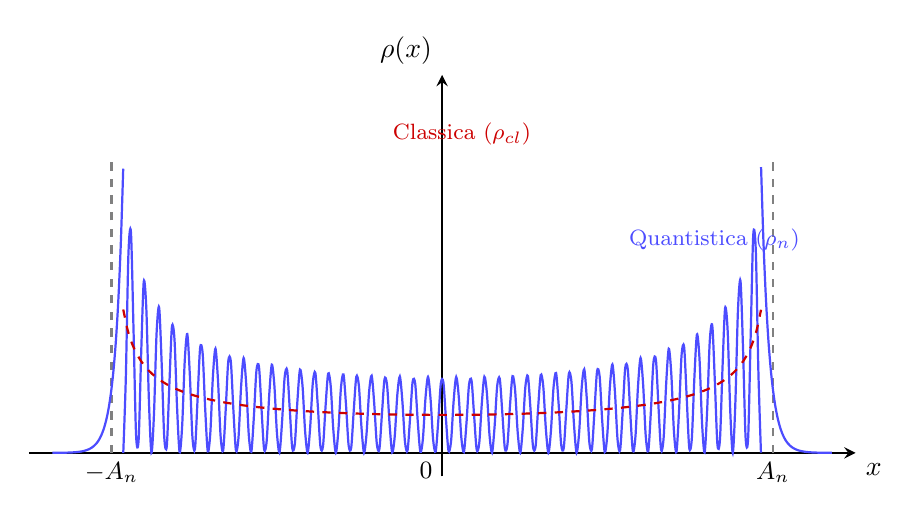
\begin{tikzpicture}[>=stealth, scale=1.5]
    \colorlet{qcolor}{blue!70!white}
    \colorlet{ccolor}{red!80!black}
    
    % Assi
    \draw[->, thick] (-3.5, 0) -- (3.5, 0) node[below right] {$x$};
    \draw[->, thick] (0, -0.2) -- (0, 3.2) node[above left] {$\rho(x)$};
    
    % Punti di inversione classici (A = 2.8)
    \draw[dashed, gray, thick] (2.8, 0) -- (2.8, 2.5);
    \draw[dashed, gray, thick] (-2.8, 0) -- (-2.8, 2.5);
    \node[below, font=\small] at (2.8, 0) {$A_n$};
    \node[below, font=\small] at (-2.8, 0) {$-A_n$};
    \node[below left, font=\small] at (0, 0) {$0$};

    % Funzione Quantistica (Inviluppo doppio della classica * oscillazione)
    % Usiamo 1500*\x in gradi: crea un'oscillazione fitta ma sotto i limiti di memoria di LaTeX.
    % Il dominio si ferma a 2.7 per evitare la divergenza esatta in 2.8.
    \draw[domain=-2.7:2.7, samples=250, smooth, qcolor, thick] 
        plot (\x, { (1.8 / sqrt(7.84 - \x*\x)) * (cos(1500 * \x))^2 });

    % Sconfinamento quantistico (le code esponenziali raccordate)
    % A x=2.7 l'inviluppo vale circa 2.42, raccordiamo l'esponenziale da lì.
    \draw[domain=2.7:3.3, samples=30, smooth, qcolor, thick] 
        plot (\x, { 2.42 * exp(-15*(\x-2.7)) });
    \draw[domain=-3.3:-2.7, samples=30, smooth, qcolor, thick] 
        plot (\x, { 2.42 * exp(15*(\x+2.7)) });

    % Funzione Classica (Media)
    % Esattamente la metà dell'inviluppo quantistico
    \draw[domain=-2.7:2.7, samples=150, smooth, ccolor, thick, dashed] 
        plot (\x, { 0.9 / sqrt(7.84 - \x*\x) });

    % Legenda
    \node[ccolor, right, font=\footnotesize] at (-0.5, 2.7) {Classica ($\rho_{cl}$)};
    \node[qcolor, right, font=\footnotesize] at (1.5, 1.8) {Quantistica ($\rho_n$)};
\end{tikzpicture}
\end{center}
Osservando il grafico, possiamo trarre considerazioni fisiche formidabili:
\begin{itemize}
    \item \textbf{Compensazione integrale:} La curva quantistica è fortemente oscillatoria: tocca continuamente lo zero (i nodi) per poi rimbalzare verso picchi massimi. Tuttavia, i picchi quantistici giacciono su una curva di \emph{inviluppo} che è esattamente il doppio della densità classica. Poiché il valore medio di un seno al quadrato su molti periodi è $1/2$, calcolando l'integrale della probabilità quantistica su un intervallino macroscopico $\Delta x$ (che comprende molte oscillazioni) si ottiene l'esatta compensazione: le aree coincidono perfettamente con l'integrale della controparte classica.
    \item \textbf{Picchi ai bordi:} Man mano che ci si avvicina ai punti di inversione $\pm A_n$, i picchi quantistici diventano sempre più alti e distanziati (la lunghezza d'onda di de Broglie aumenta perché l'impulso cinetico diminuisce). L'accumulo di probabilità quantistica ai bordi mima perfettamente la divergenza asintotica classica causata dalla velocità nulla della particella nei punti di inversione.
\end{itemize}
Per $n \to \infty$, gli strumenti di misura macroscopici non hanno la risoluzione sufficiente per distinguere i singoli nodi quantistici e misurano esclusivamente la media locale della densità di probabilità, restituendo l'esatta distribuzione classica di un oscillatore a molla.
